% Chapter Template

\chapter{Resultados} % Main chapter title

\label{Chapter5} % Change X to a consecutive number; for referencing this chapter elsewhere, use \ref{ChapterX}

\lhead{Capítulo  5. \emph{Resultados}} % Change X to a consecutive number; this is for the header on each page - perhaps a shortened title

%----------------------------------------------------------------------------------------
%	SECTION 1
%----------------------------------------------------------------------------------------

\section{Sistema final}

El sistema desarrollado proporciona las siguientes funcionalidades:

\begin{itemize}
\item Alarma:
	\begin{itemize}
	\item Monitorizado de sensores.
	\item Autenticación de usuario.
	\item Comunicación sobre IP bidireccional.
	\item Control de salidas de potencia.
	\end{itemize}
\item Servidor:
	\begin{itemize}
	\item Recepción y autenticación de alertas.
	\item Envío de alertas por \textit{E-mail}.
	\item CMS de usuarios de alarmas.
	\item Autenticación de Administradores.
	\item Notificaciones automáticas y en tiempo real.
	\end{itemize}
\item Aplicación:
	\begin{itemize}
	\item Envío de comandos configuración.
	\item Envío de comandos de control.
	\item Recepción de estado de alarma.
	\end{itemize}
\end{itemize}

Todas las funcionalidades antes descritas fueron comprobadas a nivel de código(con pruebas unitarias y de integración), como así también de nivel de usuario del sistema(pruebas de aceptación y usabilidad).\\
Se generaron varios usuarios de alarmas con su información personal desde el servidor, donde se recibieron alertas de las mismas. Se comprobó que se recibieran automáticamente y en tiempo real, al mismo tiempo que se enviaran los \textit{E-mails} correspondiente a los usuarios.Por el lado de la aplicación y la alarma, se comprobaron todas las opciones de configuración y comunicación de las mismas.

\newpage
%-----------------------------------
%	SUBSECTION 1
%-----------------------------------
\subsection{Alarma}

Una vez comprobado el correcto funcionamiento del circuito correspondiente sobre una \textit{protoboard}, se continuó con el diseño del \textit{PCB} con la herramienta de \textit{software} \textit{KiCAD}.
Con el diseño ya finalizado y comprobadas tanto las especificaciones técnicas propias como eléctricas, se construyó el circuito sobre una placa de cobre bicapa. Se procedió al soldado de componentes y posteriormente, a la comprobación de las pistas.\\
Una vez corroborado el circuito, se conectaron los sensores y se revisó que funcionasen correctamente.\\
Por el lado del \textit{software}, se verificó a través de pruebas de usuario, todos los comandos de configuración y de salida. A continuación, en la figura \ref{alarma} se muestra una fotografía del sistema embebido final.

\begin{figure}[htbp]
	\centering
		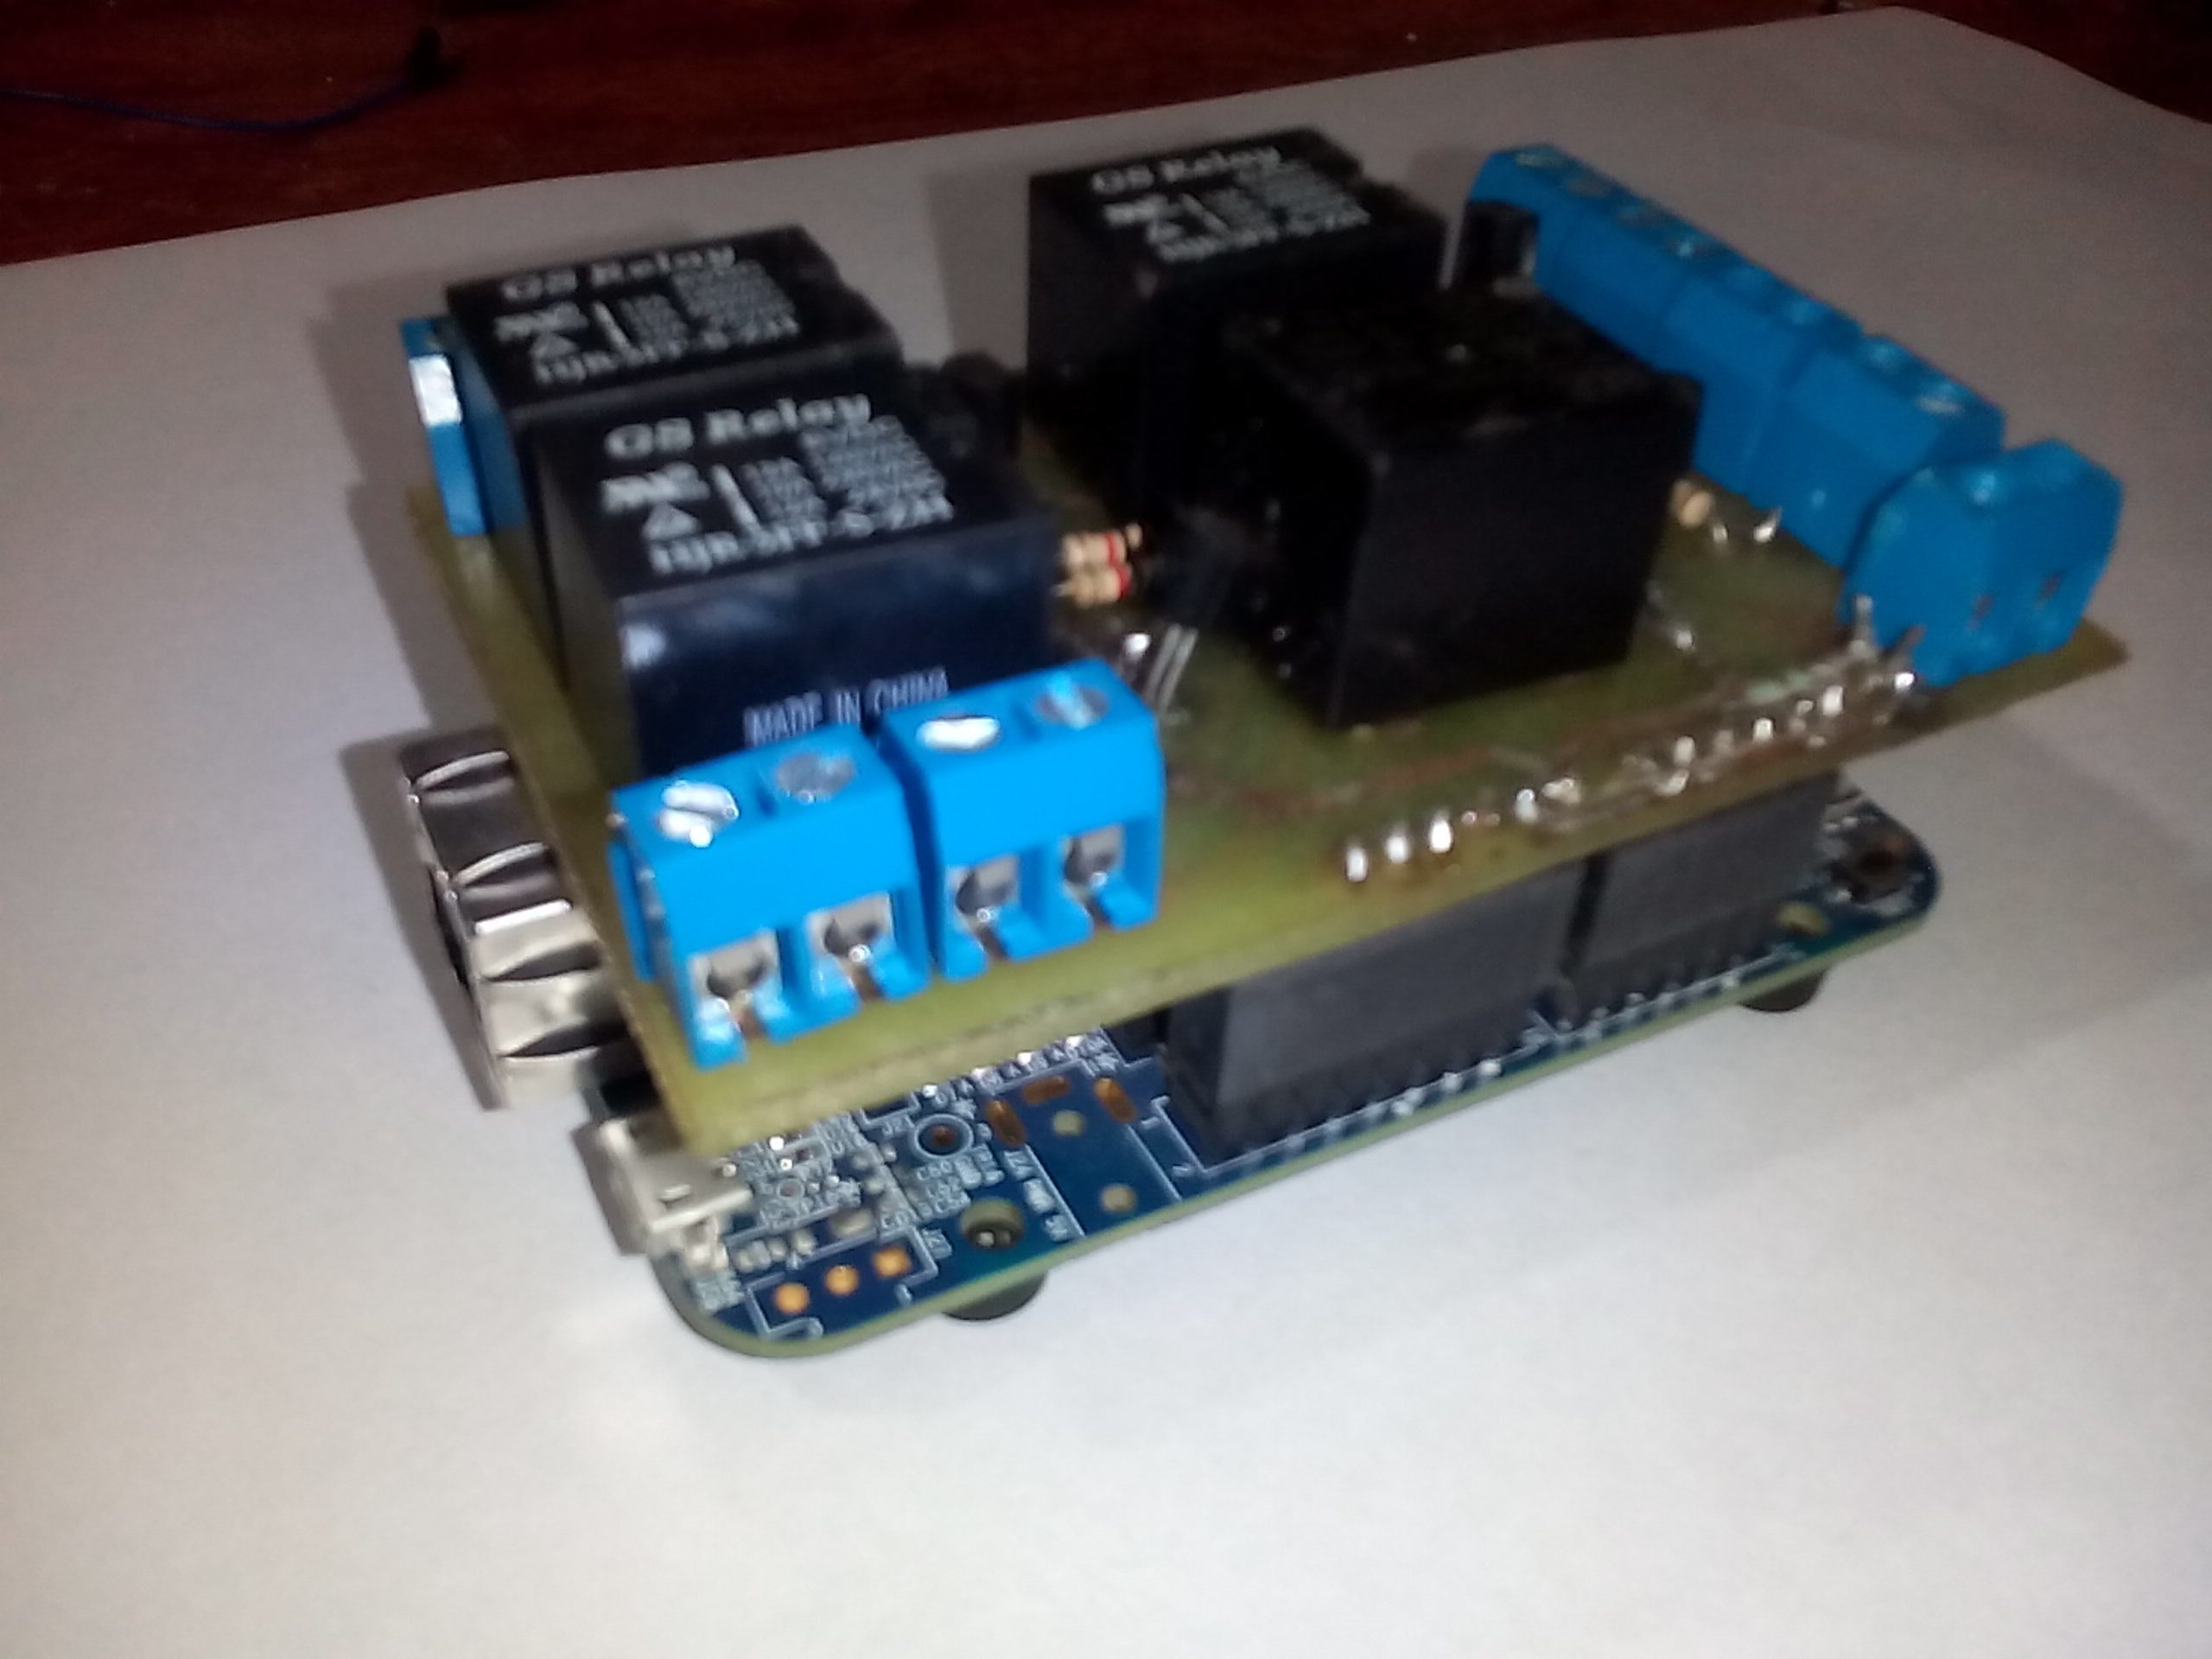
\includegraphics[width=1\textwidth]{Figures/alarma.jpg}
		\rule{35em}{1.5pt}
	\caption[Captura de Alarma final]{Captura de Alarma Final}
\label{alarma}
\end{figure}

		\subsubsection{Capacidades}
Se detallan a continuación las capacidades propias de la alama en detalle:

\begin{itemize}
\item Hasta 4 entradas de sensado de zonas.
\item Hasta 4 salidas de potencia.
\item Envío automático de alerta a servidor en Internet.
\item Comunicación bidireccional con la aplicación.
\item Autenticación de usuario y de comandos de entrada.
\end{itemize}		
		
		\subsubsection{Limitaciones}
		
Las limitaciones que presenta la alarma, tanto en \textit{Software} como en \textit{Hardware} se resumen en el siguiente apartado:

\begin{itemize}
\item Software: 
	\begin{itemize}
	\item IP de alarma fija, no configurable dinámicamente. 	
	\item Envío y recepción de mensajes sin encriptación.
	\item Información volátil, guardada en RAM.
	\end{itemize}
\item Hardware:
	\begin{itemize}
	\item Entradas no aisladas eléctricamente.
	\item Entradas limitadas a 4 sensores.
	\item Sensores únicamente del tipo \textit{ON/OFF}.
	\item Comunicación de red por cable.
	\end{itemize}
\end{itemize}
\newpage		
%-----------------------------------
%	SUBSECTION 2
%-----------------------------------

\subsection{Servidor}
Una vez constatado el correcto funcionamiento en un entorno restringido de todas las funcionalidades, se traslado el mismo a otra plataforma de \textit{Hardware}, como lo exigía uno de los requerimientos.
Finalmente, el servidor quedó montado sobre una \textit{Raspberry Pi 2}, procurando comprobar todas las funcionalidades que fueron descritas en un principio.\\


		\subsubsection{Capacidades}
A continuación se explicita las capacidades propias del servidor:

\begin{itemize}
\item Recepción, autenticación y actualización automática de las alertas.
\item Envío automático de notificaciones al usuario vía \textit{e-mail}.
\item Gestión de usuarios y alertas (\textit{CRUD}).
\item Gestión y Autenticación de administradores de sistema.
\end{itemize}
		\subsubsection{Limitaciones}
\begin{itemize}
\item Creación de niveles de jerarquías de administradores/usuarios de Sistema.
\item Un usuario por alarma.
\end{itemize}		


\newpage		
%----------------------------------------------------------------------------------------
%	SUBSECTION 3
%----------------------------------------------------------------------------------------

\subsection{Aplicación}

En este caso, se pasó por varias etapas, desde un pequeño programa en C, que simulaba el envío de comandos a la alarma, pasando posteriormente, por una aplicación genérica que realizaba las mismas acciones desde un emulador de \textit{Android}, hasta la aplicación final corriendo sobre el teléfono inteligente.

		\subsubsection{Capacidades}
\begin{itemize}
\item Envío de credenciales de autenticación.
\item Envío de comandos de configuración.
\item Envío de órdenes de accionamiento para salidas de potencia de la alarma.
\item Recepción de respuestas de la alarma.
	\begin{itemize}
	\item Resultado de comandos.
	\item Estado de alarma.
	\end{itemize}
\end{itemize}		

		\subsubsection{Limitaciones}
		
\begin{itemize}
\item Envío de comandos a IP fija.
\item No se reciben notificaciones a la aplicación.
\item No se permite editar las acciones de salida.
\end{itemize}			
	